% !TEX root = ../master.tex

\newcommand{\labelof}[1]{\underline{#1}}
\newcommand{\dlmc}[1]{\lstinline[style=dlmc]{#1}}
\newcommand{\dlmactsfor}{\dlmc{if\_acts\_for}}
\newcommand{\dlmdeclassify}{\dlmc{declassify}}
\newcommand{\dlmpc}{$\underline{pc}$}
\newcommand{\mathcomment}[1]{\color{green!50!black}{#1}}

\chapter{The Decentralized Label Model}
The Decentralized Label Model \cite{myers1997, myers1998, myers2000} is a model for ensuring information flow control in a system.
This is done by annotating source code with security policies, in the form of labels attached to data-holding constructs.
This section will present the necessary information needed to understand the implementation of \thetool.
The descriptions and definitions in this section are based on \cite{myers1997, myers1998, myers2000}.
Throughout the examples, we will use the same grammar as that used by \thetool. \mikkel{Remember to write something about the grammar/parser...}

\section{Labels and Policies}
Throughout a program, values are declared, initialized, and assigned to variables and other value-holders.
Value-holders are collectively known as \emph{slots}, which cover constructs such as variables, structs, and other storage locations.
In order to ensure that a certain assignment is legal, such that no information is unintentionally leaked, we assign \emph{labels} to slots so that their ``security'' can be compared.
This way we can ensure that an assignment is only legal in the cases where higher-security values aren't assigned to lower-security slots.
The same concept applies to more complex language constructs, such as functions (and their return values).

Each slot is associated with a label, that describes how the data in the slot can be handled.
We denote the label of slot $s$ as $\underline{s}$.
Referring to labels in this fashion serves the same purpose as letters in algebra; it allows for handling labels without knowledge about their actual value.
This proves useful as it allows for label inference and label polymorphism (see \cref{dlm:implicit_labels} and ??). \mikkel{Insert reference when written.}\mikael{Are we going to write about label polymorphism?}

For a given label it is possible to define both read (\emph{privacy}) and write (\emph{integrity}) policies.
The first represents information flow out of a system and the latter information flow into a system.
In this report only read policies will be considered.
Due to the relation between the two types of policies, we note that write policies can be ensured in a fashion similar to read policies.
Because of this we choose to simplify the scope of the report such that it only discusses read policies.

\myparagraph{Principals}
In the following, we employ the concept of \emph{principals}.
A principal (or \emph{subject}, \emph{agent}) is an entity in a system that represents some interest.
In short, principals represent real-world users or the authority under which a program/system runs.
Principals can exists in a \emph{principal hierarchy}, that describe more complex principal relationships, such as groups or roles.
\mikkel{Reminder about principal hierarchies}
In the following we make use of the special set of principals; $*$.
This set represents all principals in a system.

\myparagraph{Labels}
A label can be described as a set of policies, where a policy consists of an owner principal $o$ and a set of reader principals $r_1, r_2, \dots, r_n$.
Formally we provide the following, equivalent definition:
\begin{definition}{Labels}
A label $L$ is a set of owners $owners(L)$, and a function $readers(L, o)$ that retrieves the set of reader principals that $o$ allows to read.
Note that given this definition we have that $$o \notin owners(L) \Rightarrow readers(L, o) = *$$
\end{definition}

Owners are allowed to change their own policies within a label.
We describe how this is done in \cref{dlm:auth_and_declass}.
If an owner is not part of its own policies reader set, that owner is not allowed to read from the slot associated with the label.
He is however still allowed to change his policy.

\myparagraph{The effective reader set}
To ensure that the policies of all owners in a label are enforced, only readers that the all ``agree'' on can read from the slot associated with the label.
This is known as the \emph{effective reader set}, which is the intersection of \emph{all} reader sets of a label:
\begin{definition}{The effective reader set}
  The reader set of a label is the intersection of the reader sets of each of the labels owners reader sets:
  $$readers(L) = \bigcap_{o \in *} readers(L, o)$$
\end{definition}

\begin{example}{A label with two policies}\label{dlm:ex:simple_label}
  Below is an example of a label with two policies using the notation from above;
  $$L_1 = \{o1 \rightarrow r1, r2; o2 \rightarrow r2, r3\}$$

  The owner set of the label is $owners(L_1) = \{o1, o2\}$, and its reader sets are $readers(L_1, o1) = \{r1, r2\}, readers(L_1, o2) = \{r2, r3\}$.
  By intersecting the reader sets of the label we get the effective reader set.
  In practice we can disregard the reader set of labels that are not owners.
  Thus the effective reader set is
  $$readers(L_1) = \{r1,r2\} \cap \{r2, r3\} = \{r2\}$$
\end{example}

\section{Labels as partially ordered set}
\mikkelin{Describe why we have an interest in labels being partially ordered and then proceed to define it.}

\subsection{Composite labels}
We can construct composite labels by either joining or meeting two labels.
A composite label $L_1 \sqcup L_2$ or $L_1 \sqcap L_2$ represents nodes in a composite label structure.
To employ these labels similarly to the previously defined labels, we define the owner and reader sets of the composite labels:

\begin{definition}{Label Join}
The join operation is denoted by the operator $\sqcup$ and represents the least restrictive label that is as restrictive as either operand:
  \begin{align*}
    owners(L_1 \sqcup L_2) &= owners(L_1) \cup owners(L_2) \\
    readers(L_1 \sqcup L_2, o) &= readers(L_1, o) \cap readers(L_2, o)
  \end{align*}
\end{definition}
\begin{definition}{Label Meet}
The meet operation is denoted by the operator $\sqcap$ and represents the most restrictive label that is no more restrictive than either operand:
  \begin{align*}
    owners(L_1 \sqcap L_2) &= owners(L_1) \cap owners(L_2) \\
    readers(L_1 \sqcap L_2, o) &= readers(L_1, o) \cup readers(L_2, o)
  \end{align*}
\end{definition}

Label composition is an integral part of DLM.
Label joins allows for label evaluation of expressions, as described in \cref{semantics} and provides the means for representing implicit flows via scope blocks, as described in \cref{dlm:implicit_flows}.
Additionally when inferring labels, the meet operation allows us to infer the most restrictive label that agrees with the preexisting labels.

\subsection{Label comparison}
As mentioned above, labels provide restrictions on which principals can read from the slots that the labels ``protect''.
In order to check that security policies are enforced throughout a program, we need to be able to compare how restrictive labels are.
To do this we introduce the ``at most as restrictive as''-relation ($\sqsubseteq$) from \cite{myers1997}.

\begin{definition}{Label Restrictiveness}
  Label $L_1$ is at most as restrictive as label $L_2$ ($L_1 \sqsubseteq L_2$) if:
  \begin{align*}
    & owners(L_1) \subseteq owners(L_2) \text{ and} \\
    & \forall o \in owners(L_1) , readers(L_1, o) \supseteq readers(L_2, o)
  \end{align*}
\end{definition}

We can employ this definition to determine if two labels are equal:
If $L_1 \sqsubseteq L_2$ and $L_2 \sqsubseteq L_1$ then we must have that $L_1 = L_2$.

\myparagraph{Security class lattice}
By having this relationship between labels, we can see the set of all our labels as a partially-ordered set: a \emph{lattice}.
This means that we have a hierarchy in which the shared parent of every two individual elements is the result of a join of the two labels.
Similarly a shared child of two elements is the result of a meet of those labels.
To represent the least restrictive label of any security class lattice we have a bottom element, denoted $\bot$.
Dual to the bottom element, we also have the most restrictive label: the top element, denoted $\top$.
\Cref{dlm:lattice_fig} illustrates this label relation.

\begin{figure}
  \begin{center}
  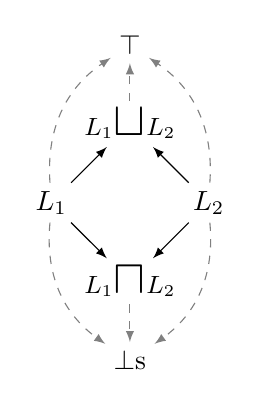
\begin{tikzpicture}[inner sep=1mm, >=latex]
    \node (l1) at (-1,0) {$L_1$};
    \node (l2) at (1,0) {$L_2$};

    \node (meet) at (0,-1) {\small $L_1$ {\LARGE $\! \sqcap \!$} $L_2$};
    \node (bot) at (0,-2) {$\bot$s};

    \node (join) at (0,1) {\small $L_1$ {\LARGE $\! \sqcup \!$} $L_2$};
    \node (top) at (0,2) {$\top$};

    \draw[->] (l1) edge (join);
    \draw[->] (l2) edge (join);
    \draw[->] (l1) edge (meet);
    \draw[->] (l2) edge (meet);

    \draw[->, dashed, gray] (l1) edge [bend left] (top);
    \draw[->, dashed, gray] (join) edge (top);
    \draw[->, dashed, gray] (l2) edge [bend right] (top);

    \draw[->, dashed, gray] (l1) edge [bend right] (bot);
    \draw[->, dashed, gray] (meet) edge (bot);
    \draw[->, dashed, gray] (l2) edge [bend left] (bot);
  \end{tikzpicture}
  \caption{Abstraction of security lattice}
  \label{dlm:lattice_fig}
  \end{center}
\end{figure}

\section{Implicit flows}\label{dlm:implicit_flows}
When assigning a value to a slot, possibly from another slot, it is an explicit flow.
In addition to explicit flows, it is also possible to have implicit flows throughout a program, due to conditional control structures (such as loops).
For whatever assignments we would do inside a block (or within a deeper block hierarchy) we need to take the predicates of these blocks into consideration.
This is done by adding the concept of \emph{program counter labels}, denoted \dlmpc.
For each scope we will have an implicit \dlmpc, depending on the surrounding predicates' labels.

\begin{example}{Implicit leak}\label{dlm:ex:implicit_leak}
  Consider the following program (each line commented with the current \dlmpc):
  \begin{lstlisting}[style=dlmc]
int {{a->z,y}} val = 0;   // $\mathcomment{\bot}$
int {{a->y}} cond = 1;    // $\mathcomment{\bot}$
if (cond) {
  val++;                  // $\mathcomment{\bot \sqcup \{a \rightarrow y\}}$
}
return val;               // $\mathcomment{\bot}$
  \end{lstlisting}
  In this example we would have an implicit leak of \dlmc{cond}, by way of \dlmc{val}.
  This is due to the assignment of \dlmc{val} inside of the \dlmc{if}-statement, as \dlmpc~ is increased to the join of the outer scope ($\bot$) and the label of the scope's predicate (\labelof{\dlmc{cond}}).
  For this program to pass \thetool, we would have to add a more strict policy to \dlmc{val}, so that it could match the policy of \dlmc{cond}.
\end{example}

\subsection{Authority and declassification}\label{dlm:auth_and_declass}
In order to avoid mishaps by setting certain policies too lax, so that certain flows are permitted, we can temporarily set some policies to be more strict, and then only relax (\emph{declassify}) them when we really need to.
In order to do this, the concept of \emph{authority} is introduced.

At any point during execution of a program, it will have a \emph{true authority}, which is the maximal authority by which the program can carry out operations.
Whenever we call a function, we can do this with a certain authority, corresponding to running that method with the authority of a specific principal or principals.
However, in order to take advantage of this given authority, we need to explicitly claim it.
This is done by using the \dlmactsfor\dlmc{(a, b) \{ stmts \}} statement, where $a$ is the principal (typically the function itself) trying to obtain the authority of $b$.
Only after calling this function will we obtain the \emph{effective authority} to act for $b$, enabling us to carry out the statements within the \dlmactsfor~ block that would normally only be permissible for $b$ itself.

If the check passed, the \dlmc{stmt} block will be executed under the the newly established authority.
If the check fails, the block is not executed.

With $b$ in the effective authority we can perform declassification -- deliberately and explicitly relaxing the security policies in which $b$ is owner.
This is done by calling the \dlmdeclassify\dlmc{(v, l)} function, with a slot $v$ and a new label $l$ as inputs, returning the value $v$ relabeled to $l$.
The relabeling by declassification rule (the inference rule) is defined as follows:

\begin{definition}{Relabeling by declassification}
  Let $P$ denote the set of principals in the current authority, then
  \[
  \frac
  {
    \splitfrac
    {
      L_A = \mathlarger\sqcupl_{p \in P} \{p \rightarrow \emptyset \}
    }
    {
      L_1 \sqsubseteq L_2 \sqcup L_A
    }
  }
  {
    L_1 \text{ may be declassified to } L_2
  }
  \]
\end{definition}

The combination of these two concepts, \dlmactsfor~ and \dlmdeclassify, is especially useful when we have sensitive inputs to a method and want to carry out our calculations without the fear of neither explicit or implicit leakage.
This way we can keep our strict policies throughout the calculations of the method and only relax the label once we want to return the result.

\begin{example}{Temporarily restricting a label}
  Building on \cref{dlm:ex:implicit_leak}, we can set the label for \dlmc{val} to match that of \dlmc{cond}, and then only relax that label when we need to return \dlmc{val}, ensuring that we have the ability to do so:
  \begin{lstlisting}[style=dlmc]
int {{a->y}} val = 0;
int {{a->y}} cond = 1;
if (cond) {
  val++;
}
if_acts_for(this, a) {
  return declassify(x, {{a->y,z}});
}
return -1;
  \end{lstlisting}
  While we still leak some information about \dlmc{cond}, we now do it explicitly.
\end{example}

\section{Label-checking and inference}
